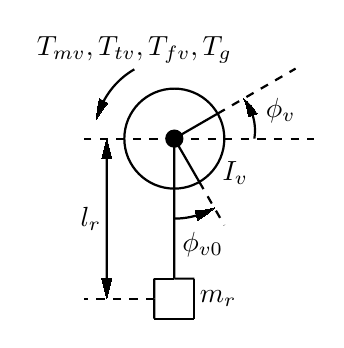
\begin{tikzpicture}[scale=2.54]
% dpic version 2015.10.28 option -g for TikZ and PGF 1.01
\ifx\dpiclw\undefined\newdimen\dpiclw\fi
\global\def\dpicdraw{\draw[line width=\dpiclw]}
\global\def\dpicstop{;}
\dpiclw=0.8bp
\dpicdraw (0.25,0) circle (0.098425in)\dpicstop
\draw (0.463388,-0.088388) node[below right=-1.5bp]{$I_v$};
\dpicdraw[fill=black](0.25,0) circle (0.015748in)\dpicstop
\dpicdraw[dashed](0.25,0)
 --(0.95,0)\dpicstop
\dpicdraw (0.25,0)
 --(0.466508,0.124997)\dpicstop
\dpicdraw[dashed](0.466508,0.124997)
 --(0.856223,0.349991)\dpicstop
\filldraw[line width=0bp](0.642269,0.116546)
 --(0.620058,0.109531)
 ..controls (0.617936,0.140904) and (0.609914,0.171595)
 ..(0.596413,0.199995)
 ..controls (0.624131,0.179484) and (0.647306,0.15346)
 ..(0.664481,0.123561)
 --(0.642269,0.116546)\dpicstop
\dpicdraw[line width=0.8bp](0.622011,0.162387)
 ..controls (0.649424,0.112977) and (0.65929,0.055737)
 ..(0.65,0)\dpicstop
\draw (0.78126,0.142346) node{$\phi_v$};
\dpicdraw (0.15003,-0.800009)
 --(0.150035,-0.900009)\dpicstop
\dpicdraw (0.150035,-0.900009)
 --(0.250035,-0.900009)\dpicstop
\dpicdraw (0.250035,-0.900009)
 --(0.350035,-0.900009)\dpicstop
\dpicdraw (0.350035,-0.900009)
 --(0.350039,-0.800009)\dpicstop
\dpicdraw (0.350039,-0.800009)
 --(0.350044,-0.700009)\dpicstop
\dpicdraw (0.350044,-0.700009)
 --(0.250044,-0.7)\dpicstop
\dpicdraw (0.250044,-0.7)
 --(0.150044,-0.699991)\dpicstop
\dpicdraw (0.150044,-0.699991)
 --(0.150049,-0.799991)\dpicstop
\dpicdraw (0.250044,-0.7)
 --(0.25,0)\dpicstop
\draw (0.350044,-0.8) node[right=-1.5bp]{$m_r$};
\dpicdraw[dashed](0.15003,-0.800009)
 --(-0.199963,-0.8)\dpicstop
\dpicdraw[dashed](0.25,0)
 --(-0.2,0)\dpicstop
\filldraw[line width=0bp](-0.112468,-0.700001)
 --(-0.087463,-0.8)
 --(-0.062468,-0.699999) --cycle\dpicstop
\filldraw[line width=0bp](-0.062495,-0.099999)
 --(-0.0875,0)
 --(-0.112495,-0.100001) --cycle\dpicstop
\dpicdraw (-0.087464,-0.777094)
 --(-0.087499,-0.022906)\dpicstop
\draw (-0.087481,-0.4) node[left=-1.5bp]{$l_r$};
\dpicdraw (0.25,0)
 --(0.375007,-0.216502)\dpicstop
\dpicdraw[dashed](0.375007,-0.216502)
 --(0.500013,-0.433005)\dpicstop
\filldraw[line width=0bp](0.360889,-0.384675)
 --(0.354231,-0.361579)
 ..controls (0.386655,-0.360424) and (0.418818,-0.355328)
 ..(0.450011,-0.346404)
 ..controls (0.425276,-0.370321) and (0.397559,-0.390948)
 ..(0.367546,-0.407772)
 --(0.360889,-0.384675)\dpicstop
\dpicdraw[line width=0.8bp](0.409313,-0.366905)
 ..controls (0.359043,-0.388733) and (0.304823,-0.399997)
 ..(0.250019,-0.4)\dpicstop
\draw (0.392371,-0.531254) node{$\phi_{v0}$};
\filldraw[line width=0bp](-0.103189,0.188492)
 --(-0.081983,0.177175)
 ..controls (-0.103746,0.153112) and (-0.122501,0.126492)
 ..(-0.137835,0.097899)
 ..controls (-0.137756,0.132306) and (-0.133239,0.166559)
 ..(-0.124394,0.199809)
 --(-0.103189,0.188492)\dpicstop
\dpicdraw[line width=0.8bp](-0.124183,0.141376)
 ..controls (-0.091534,0.22779) and (-0.029981,0.300239)
 ..(0.050021,0.346423)\dpicstop
\draw (0.050021,0.346423) node[above=-1.5bp]{$T_{mv},T_{tv},T_{fv},T_g$};
\end{tikzpicture}
